% Options for packages loaded elsewhere
\PassOptionsToPackage{unicode}{hyperref}
\PassOptionsToPackage{hyphens}{url}
%
\documentclass[
]{article}
\usepackage{amsmath,amssymb}
\usepackage{lmodern}
\usepackage{iftex}
\ifPDFTeX
  \usepackage[T1]{fontenc}
  \usepackage[utf8]{inputenc}
  \usepackage{textcomp} % provide euro and other symbols
\else % if luatex or xetex
  \usepackage{unicode-math}
  \defaultfontfeatures{Scale=MatchLowercase}
  \defaultfontfeatures[\rmfamily]{Ligatures=TeX,Scale=1}
\fi
% Use upquote if available, for straight quotes in verbatim environments
\IfFileExists{upquote.sty}{\usepackage{upquote}}{}
\IfFileExists{microtype.sty}{% use microtype if available
  \usepackage[]{microtype}
  \UseMicrotypeSet[protrusion]{basicmath} % disable protrusion for tt fonts
}{}
\makeatletter
\@ifundefined{KOMAClassName}{% if non-KOMA class
  \IfFileExists{parskip.sty}{%
    \usepackage{parskip}
  }{% else
    \setlength{\parindent}{0pt}
    \setlength{\parskip}{6pt plus 2pt minus 1pt}}
}{% if KOMA class
  \KOMAoptions{parskip=half}}
\makeatother
\usepackage{xcolor}
\IfFileExists{xurl.sty}{\usepackage{xurl}}{} % add URL line breaks if available
\IfFileExists{bookmark.sty}{\usepackage{bookmark}}{\usepackage{hyperref}}
\hypersetup{
  pdftitle={Finding Out If People Are Getting Divorced Due to the Lockdown Caused by the COVID-19 Pandemic.},
  pdfauthor={Min Chang},
  hidelinks,
  pdfcreator={LaTeX via pandoc}}
\urlstyle{same} % disable monospaced font for URLs
\usepackage[margin=1in]{geometry}
\usepackage{longtable,booktabs,array}
\usepackage{calc} % for calculating minipage widths
% Correct order of tables after \paragraph or \subparagraph
\usepackage{etoolbox}
\makeatletter
\patchcmd\longtable{\par}{\if@noskipsec\mbox{}\fi\par}{}{}
\makeatother
% Allow footnotes in longtable head/foot
\IfFileExists{footnotehyper.sty}{\usepackage{footnotehyper}}{\usepackage{footnote}}
\makesavenoteenv{longtable}
\usepackage{graphicx}
\makeatletter
\def\maxwidth{\ifdim\Gin@nat@width>\linewidth\linewidth\else\Gin@nat@width\fi}
\def\maxheight{\ifdim\Gin@nat@height>\textheight\textheight\else\Gin@nat@height\fi}
\makeatother
% Scale images if necessary, so that they will not overflow the page
% margins by default, and it is still possible to overwrite the defaults
% using explicit options in \includegraphics[width, height, ...]{}
\setkeys{Gin}{width=\maxwidth,height=\maxheight,keepaspectratio}
% Set default figure placement to htbp
\makeatletter
\def\fps@figure{htbp}
\makeatother
\setlength{\emergencystretch}{3em} % prevent overfull lines
\providecommand{\tightlist}{%
  \setlength{\itemsep}{0pt}\setlength{\parskip}{0pt}}
\setcounter{secnumdepth}{5}
\newlength{\cslhangindent}
\setlength{\cslhangindent}{1.5em}
\newlength{\csllabelwidth}
\setlength{\csllabelwidth}{3em}
\newlength{\cslentryspacingunit} % times entry-spacing
\setlength{\cslentryspacingunit}{\parskip}
\newenvironment{CSLReferences}[2] % #1 hanging-ident, #2 entry spacing
 {% don't indent paragraphs
  \setlength{\parindent}{0pt}
  % turn on hanging indent if param 1 is 1
  \ifodd #1
  \let\oldpar\par
  \def\par{\hangindent=\cslhangindent\oldpar}
  \fi
  % set entry spacing
  \setlength{\parskip}{#2\cslentryspacingunit}
 }%
 {}
\usepackage{calc}
\newcommand{\CSLBlock}[1]{#1\hfill\break}
\newcommand{\CSLLeftMargin}[1]{\parbox[t]{\csllabelwidth}{#1}}
\newcommand{\CSLRightInline}[1]{\parbox[t]{\linewidth - \csllabelwidth}{#1}\break}
\newcommand{\CSLIndent}[1]{\hspace{\cslhangindent}#1}
\usepackage{float} \floatplacement{figure}{H}
\usepackage{booktabs}
\usepackage{longtable}
\usepackage{array}
\usepackage{multirow}
\usepackage{wrapfig}
\usepackage{float}
\usepackage{colortbl}
\usepackage{pdflscape}
\usepackage{tabu}
\usepackage{threeparttable}
\usepackage{threeparttablex}
\usepackage[normalem]{ulem}
\usepackage{makecell}
\usepackage{xcolor}
\ifLuaTeX
  \usepackage{selnolig}  % disable illegal ligatures
\fi

\title{Finding Out If People Are Getting Divorced Due to the Lockdown Caused by the COVID-19 Pandemic.\thanks{Code and data are available at: \url{https://github.com/min-315/Divorces-During-Lockdown.git}}}
\usepackage{etoolbox}
\makeatletter
\providecommand{\subtitle}[1]{% add subtitle to \maketitle
  \apptocmd{\@title}{\par {\large #1 \par}}{}{}
}
\makeatother
\subtitle{Observing the number divorces in Canada from 2019 to 2021.}
\author{Min Chang}
\date{30 April 2022}

\begin{document}
\maketitle
\begin{abstract}
Using the data from both Open Data Toronto and Open Data Government of Canada, this report looks into registered marriage and divorce cases that may have occurred due to the COVID-19 Lockdown. The lockdown has made people to stay with their family or partners every day at their homes to lower the COVID-19 cases. However, the result of the lockdown were not only lowered COVID-19 cases but also changes in martial statuses from either married or divorced. Further analysis of the data was done to yield a better understanding to the changes in martial statuses after the lockdown.

\par

\textbf{Keywords:} COVID-19, Lockdown, Marriage, Divorce, Toronto, Canada, Open Data Toronto, Open Data Government of Canada
\end{abstract}

\tableofcontents

\hypertarget{introduction}{%
\section{Introduction}\label{introduction}}

The COVID-19 pandemic has lead to a lock-down that caused the world,including Canada, to momentarily stop from social gatherings, eating at restaurants, shopping, and any occasions that may involve groups of people in one area. To prevent the virus from spreading further, the Canadian Government requested people to remain in their homes until the COVID-19 cases flattened and was safe for people to go back to their normal daily lives. However, the lock-down meant people had to constantly be in close contact with their families and/or partners in the same space for several days until the lock-down was done (Liu 2020).

As the lock-down made people to stay at their homes, some took the opportunity to catch up with their families and/or partners as education and work has also shifted to remote, people had more flexibility with their time. However, with limited space and repeatedly interacting with families and/or partners can become tiring and irritable. Especially, with married couples, there has been information married couples were getting divorced after the lock-down was over (Savage 2020).

Therefore, through this report, we will take a look into divorce cases in Canada to see if a lot of people are actually getting divorced after the lock-down. We then will take a look at registered marriage cases in Toronto to see the differences in the number of marriages versus divorces to see which relationship change was the most effected by the lock-down.

\hypertarget{data}{%
\section{Data}\label{data}}

\hypertarget{source}{%
\subsection{Source}\label{source}}

Two different data-sets are used for this report. The data-set for divorce cases in Canada is retrieved from Open Data Government of Canada which includes data regarding people who have gotten married or divorced from 1970 to 2020; it also includes geographic data of different provinces in Canada (Canada 2022). The other data-set is the registered marriage cases in Toronto that is retrieved from Open Data Toronto which includes data on registered marriages in different cities in Ontario, Canada (Toronto 2022). Using those two data-sets, popular information regarding increasing cases of divorce between married couples after the lock-down can be observed and will also compare the data with number of registered marriages during the similar time period of people getting divorced to see if it caused any changes to people who were about to get married.

\hypertarget{data-organization}{%
\subsection{Data Organization}\label{data-organization}}

To analyze the two data-sets, the \texttt{R\ programming\ language}(R Core Team 2021) was used for statistical computing and graphics.
The \texttt{opendatatoronto}(Gelfand 2020) was used to access the City of Toronto Open Data portal. The \texttt{tidyverse} (Wickham et al. 2019) package was downloaded to use the other R packages. The \texttt{dplyr} (Wickham et al. 2021) was downloaded to help have freedom controlling the variables in the data. The \texttt{readr} (Wickham et al. 2022) was downloaded to read rectangular data, such as csv files, in a convenient and fast manner. The \texttt{kableExtra} (Zhu 2021) was downloaded to help construct tables. The \texttt{ggplot2} (Wickham 2016) was downloaded ot help construct any style of graphs. The \texttt{forcats} (Wickham 2021) was downloaded to work with categorical variables. The \texttt{tibbletime} (Vaughan and Dancho 2020) was downloaded to easily control the time within data-sets. Lastly, the \texttt{knitr} (Xie 2021) was downloaded to allow data to be processed into various document formats.

\hypertarget{result}{%
\section{Result}\label{result}}

With several \texttt{R\ packages} downloaded, the two data-sets were cleaned to only have variables that are useful and to make it easier to observe.

\begin{table}[H]

\caption{\label{tab:table}Divorced Cases in Canada from 2019 to 2020}
\centering
\begin{tabular}[t]{ccc}
\toprule
Year & Geographic & Sex\\
\midrule
2019 & Canada & Both sexes\\
2019 & Canada & Both sexes\\
2020 & Canada & Both sexes\\
2020 & Canada & Both sexes\\
\bottomrule
\end{tabular}
\end{table}

Table.\ref{tab:table} is showing divorce cases that were filed in Canada between 2019 and 2020. Before Table.\ref{tab:table} was constructed, the original data-set included empty and unclear variables that did not serve any purpose for this report.The data-set is also quite big as it includes divorce cases starting from 1970 and divorce cases that were filed from different provinces in Canada.Thus, with the downloaded R packages, 16 variables were cleaned into 3 variables and the time period was also filtered to be between 2019 to 2020. In addition, the geographic area was filtered to only Canada because the table would have become too complex to observe and it made more sense to see the overall divorce cases in Canada as divorces do not occur in one specific area. Lastly, the data-set was only updated until 2020, thus the data is missing data on 2021 which would been much better comparing with Figure.\ref{fig:line}. Moreover, the data-set is unclear with the number of divorce cases as there is no number that indicates the amount of people who got divorced in 2019 and 2020.

\begin{figure}
\centering
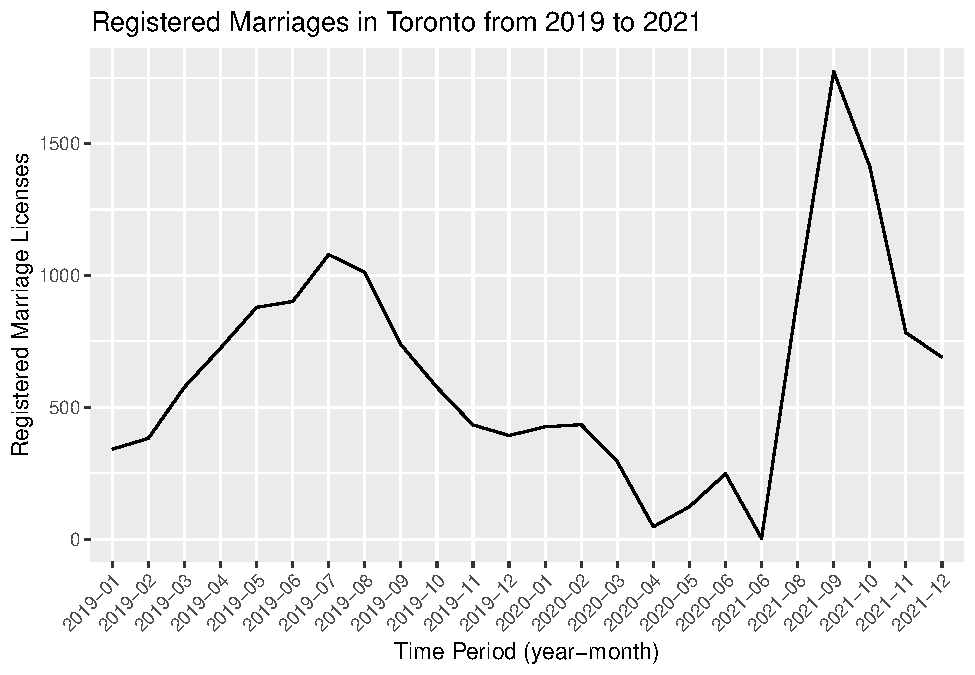
\includegraphics{Divorces-During-COVID-19_files/figure-latex/line-1.pdf}
\caption{\label{fig:line}Number of Registered Marriage Licenses From 2019 to 2021}
\end{figure}

Figure.\ref{fig:line} is a line graph that is showing the number of registered marriage licenses and the changes from 2019 to 2021. Compared to Table.\ref{tab:table}'s data-set, Figure.\ref{fig:line}'s data-set has less variables to clean and did not contain variables that were empty or were meaningless for this report. The variables that were filtered were the cities and time period the marriage licenses were registered. This data-set was constructed to be a line graph to observe the number of people registering their marriages from 2019 to 2021. The data-set included 2022 data as well but 2022 is when the lock-down was no longer applied in any provinces in Canada like Ontario, therefore it would have not help support the purpose of this report.

After creating the table (Table.\ref{tab:table}) and graph (Figure.\ref{fig:line}), with the data available it is evident that there are more people getting married than getting divorced. There are articles that a lot more people are getting divorced after the lock-down as people were getting tired of constantly being in close contact with their family and/or partners in a limited space (Liu 2020). On top of close contact, people were becoming more aware of their mental health after realizing how tiring it is to repeatedly experience days that feel the same (Savage 2020). On the other hand, there are relationships that became stronger after lock-down as they were able to spend more time to learn more about each other and figure out various ways to understand each other (Bowden 2020). Overall, the lock-down did effect relationships to change their status to either married or divorced.

\hypertarget{discussion}{%
\section{Discussion}\label{discussion}}

There was an expectation of high divorce cases with married couples other than having to constantly be in close contact with each other. Couples with kid(s) had more work in their homes as the lock-down caused school to be delivered online making parents having to take care of their kids while doing their own work (Savage 2020). Most households, either parents can focus more on housework when kids are at school as parents do not have to stop mid-way to help take care of their (kid)s. Especially with parents who do not have their partners to help with the household would have struggled more to take care of their kids and the household work at the same time. After the lock-down was over, women were the ones who initiated the divorce as they were still experiencing ``disproportionate share of housework and childcare'' (Savage 2020). However, unlike the articles about divorces after lock-down, Table.\ref{tab:table} is showing approximately four cases of divorces in Canada. The four divorce cases in Canada could either mean 40 or 4 people for each case, but as the data itself was unclear to begin with, it is hard to decipher.

On the other hand, Figure.\ref{fig:line} is showing a great increase in registered marriage licenses between 2021 June to September which was the time period where lock-down was just over. Even though there were couples that realized their relationship could not move any further, there were also couples discovering life-long partners. Some people thought the lock-down was the perfect timing to lock their relationships with their partners as their love towards each other were validated by taking the extra time they had in their homes to know more about each other (Bowden 2020). According to (Sachser et al. 2021), during the lock-down younger couples' relationship quality actually improved much better leading to marriage, when older couple's relationship quality deteriorated leading to divorces. With that information in mind, there can be an assumption that Table.\ref{tab:table} is showing the data of divorce cases that were filed after lock-down would be older couples rather than younger couples.

\hypertarget{further-improvements}{%
\subsection{Further Improvements}\label{further-improvements}}

After analyzing the data with supporting articles, the report would have been more engaging with the comparison of number of females and males initiating divorces.The supporting articles often mention women are the people who initiate divorces and felt the most pressure during the lock-down (Savage 2020).

\newpage

\hypertarget{references}{%
\section*{References}\label{references}}
\addcontentsline{toc}{section}{References}

\hypertarget{refs}{}
\begin{CSLReferences}{1}{0}
\leavevmode\vadjust pre{\hypertarget{ref-Bowden}{}}%
Bowden, Olivia. 2020. {``These Canadians Popped the Question During a Pandemic: {`It Made It Even Better'}.''} \url{https://globalnews.ca/news/6859000/engagements-during-coronavirus/}.

\leavevmode\vadjust pre{\hypertarget{ref-divorce}{}}%
Canada, Government of. 2022. \emph{Mean Age and Median Age at Divorce and at Marriage, for Persons Who Divorced in a Given Year, by Sex or Gender}. \url{https://open.canada.ca/data/en/dataset/82cc8f33-3b40-4a57-83d1-b8059a12f742}.

\leavevmode\vadjust pre{\hypertarget{ref-opendata}{}}%
Gelfand, Sharla. 2020. \emph{Opendatatoronto: Access the City of Toronto Open Data Portal}. \url{https://CRAN.R-project.org/package=opendatatoronto}.

\leavevmode\vadjust pre{\hypertarget{ref-Liu}{}}%
Liu, Yi-Ling. 2020. {``Is Covid-19 Changing Our Relationships?''} \url{https://www.bbc.com/future/article/20200601-how-is-covid-19-is-affecting-relationships}.

\leavevmode\vadjust pre{\hypertarget{ref-R}{}}%
R Core Team. 2021. \emph{R: A Language and Environment for Statistical Computing}. Vienna, Austria: R Foundation for Statistical Computing. \url{https://www.R-project.org/}.

\leavevmode\vadjust pre{\hypertarget{ref-Sacher}{}}%
Sachser, Cedric, Gabriel Olaru, Elisa Pfeiffer, Elmar Brähler, Vera Clemens, Miriam Rassenhofer Andreas Witt, and Jörg M.Fegert. 2021. {``The Immediate Impact of Lockdown Measures on Mental Health and Couples' Relationships During the COVID-19 Pandemic - Results of a Representative Population Survey in Germany.''} \emph{Social Science \& Medicine} 278. https://doi.org/\url{https://doi.org/10.1016/j.socscimed.2021.113954}.

\leavevmode\vadjust pre{\hypertarget{ref-Savage}{}}%
Savage, Maddy. 2020. {``Why the Pandemic Is Causing Spikes in Break-Ups and Divorces.''} \url{https://www.bbc.com/worklife/article/20201203-why-the-pandemic-is-causing-spikes-in-break-ups-and-divorces}.

\leavevmode\vadjust pre{\hypertarget{ref-registered}{}}%
Toronto, City of. 2022. \emph{About Marriage Licence Statistics}. \url{https://open.toronto.ca/dataset/marriage-licence-statistics/}.

\leavevmode\vadjust pre{\hypertarget{ref-tibbletime}{}}%
Vaughan, Davis, and Matt Dancho. 2020. \emph{Tibbletime: Time Aware Tibbles}. \url{https://cran.r-project.org/web/packages/tibbletime/index.html}.

\leavevmode\vadjust pre{\hypertarget{ref-ggplot2}{}}%
Wickham, Hadley. 2016. \emph{Ggplot2: Elegant Graphics for Data Analysis}. Springer-Verlag New York. \url{https://ggplot2.tidyverse.org}.

\leavevmode\vadjust pre{\hypertarget{ref-cats}{}}%
---------. 2021. \emph{Forcats: Tools for Working with Categorical Variables (Factors)}. \url{https://CRAN.R-project.org/package=forcats}.

\leavevmode\vadjust pre{\hypertarget{ref-tidyverse}{}}%
Wickham, Hadley, Mara Averick, Jennifer Bryan, Winston Chang, Lucy D'Agostino McGowan, Romain François, Garrett Grolemund, et al. 2019. {``Welcome to the {tidyverse}.''} \emph{Journal of Open Source Software} 4 (43): 1686. \url{https://doi.org/10.21105/joss.01686}.

\leavevmode\vadjust pre{\hypertarget{ref-dplyr}{}}%
Wickham, Hadley, Romain François, Lionel Henry, and Kirill Müller. 2021. \emph{Dplyr: A Grammar of Data Manipulation}. \url{https://CRAN.R-project.org/package=dplyr}.

\leavevmode\vadjust pre{\hypertarget{ref-readr}{}}%
Wickham, Hadley, Jim Hester, Romain Francois, Jennifer Bryan, Shelby Bearrows, RStudio, Jukka Jylänki, and Mikkel Jørgensen. 2022. \emph{Readr: Read Rectangular Text Data}. \url{https://cran.r-project.org/web/packages/readr/index.html}.

\leavevmode\vadjust pre{\hypertarget{ref-knitr}{}}%
Xie, Yihui. 2021. \emph{Knitr: A General-Purpose Package for Dynamic Report Generation in r}.

\leavevmode\vadjust pre{\hypertarget{ref-kableextra}{}}%
Zhu, Hao. 2021. \emph{kableExtra: Construct Complex Table with 'Kable' and Pipe Syntax}. \url{https://CRAN.R-project.org/package=kableExtra}.

\end{CSLReferences}

\end{document}
